% Options for packages loaded elsewhere
\PassOptionsToPackage{unicode}{hyperref}
\PassOptionsToPackage{hyphens}{url}
%
\documentclass[
]{article}
\usepackage{amsmath,amssymb}
\usepackage{lmodern}
\usepackage{iftex}
\ifPDFTeX
  \usepackage[T1]{fontenc}
  \usepackage[utf8]{inputenc}
  \usepackage{textcomp} % provide euro and other symbols
\else % if luatex or xetex
  \usepackage{unicode-math}
  \defaultfontfeatures{Scale=MatchLowercase}
  \defaultfontfeatures[\rmfamily]{Ligatures=TeX,Scale=1}
\fi
% Use upquote if available, for straight quotes in verbatim environments
\IfFileExists{upquote.sty}{\usepackage{upquote}}{}
\IfFileExists{microtype.sty}{% use microtype if available
  \usepackage[]{microtype}
  \UseMicrotypeSet[protrusion]{basicmath} % disable protrusion for tt fonts
}{}
\makeatletter
\@ifundefined{KOMAClassName}{% if non-KOMA class
  \IfFileExists{parskip.sty}{%
    \usepackage{parskip}
  }{% else
    \setlength{\parindent}{0pt}
    \setlength{\parskip}{6pt plus 2pt minus 1pt}}
}{% if KOMA class
  \KOMAoptions{parskip=half}}
\makeatother
\usepackage{xcolor}
\IfFileExists{xurl.sty}{\usepackage{xurl}}{} % add URL line breaks if available
\IfFileExists{bookmark.sty}{\usepackage{bookmark}}{\usepackage{hyperref}}
\hypersetup{
  pdftitle={The French Covid-19 vaccination policy did not solve vaccination inequities: a nationwide longitudinal study on 64.5 million individuals},
  pdfauthor={F. Débarre, E. Lecoeur, L. Guimier, M. Jauffret-Roustide, A.-S. Jannot},
  hidelinks,
  pdfcreator={LaTeX via pandoc}}
\urlstyle{same} % disable monospaced font for URLs
\usepackage[margin=1in]{geometry}
\usepackage{color}
\usepackage{fancyvrb}
\newcommand{\VerbBar}{|}
\newcommand{\VERB}{\Verb[commandchars=\\\{\}]}
\DefineVerbatimEnvironment{Highlighting}{Verbatim}{commandchars=\\\{\}}
% Add ',fontsize=\small' for more characters per line
\usepackage{framed}
\definecolor{shadecolor}{RGB}{248,248,248}
\newenvironment{Shaded}{\begin{snugshade}}{\end{snugshade}}
\newcommand{\AlertTok}[1]{\textcolor[rgb]{0.94,0.16,0.16}{#1}}
\newcommand{\AnnotationTok}[1]{\textcolor[rgb]{0.56,0.35,0.01}{\textbf{\textit{#1}}}}
\newcommand{\AttributeTok}[1]{\textcolor[rgb]{0.77,0.63,0.00}{#1}}
\newcommand{\BaseNTok}[1]{\textcolor[rgb]{0.00,0.00,0.81}{#1}}
\newcommand{\BuiltInTok}[1]{#1}
\newcommand{\CharTok}[1]{\textcolor[rgb]{0.31,0.60,0.02}{#1}}
\newcommand{\CommentTok}[1]{\textcolor[rgb]{0.56,0.35,0.01}{\textit{#1}}}
\newcommand{\CommentVarTok}[1]{\textcolor[rgb]{0.56,0.35,0.01}{\textbf{\textit{#1}}}}
\newcommand{\ConstantTok}[1]{\textcolor[rgb]{0.00,0.00,0.00}{#1}}
\newcommand{\ControlFlowTok}[1]{\textcolor[rgb]{0.13,0.29,0.53}{\textbf{#1}}}
\newcommand{\DataTypeTok}[1]{\textcolor[rgb]{0.13,0.29,0.53}{#1}}
\newcommand{\DecValTok}[1]{\textcolor[rgb]{0.00,0.00,0.81}{#1}}
\newcommand{\DocumentationTok}[1]{\textcolor[rgb]{0.56,0.35,0.01}{\textbf{\textit{#1}}}}
\newcommand{\ErrorTok}[1]{\textcolor[rgb]{0.64,0.00,0.00}{\textbf{#1}}}
\newcommand{\ExtensionTok}[1]{#1}
\newcommand{\FloatTok}[1]{\textcolor[rgb]{0.00,0.00,0.81}{#1}}
\newcommand{\FunctionTok}[1]{\textcolor[rgb]{0.00,0.00,0.00}{#1}}
\newcommand{\ImportTok}[1]{#1}
\newcommand{\InformationTok}[1]{\textcolor[rgb]{0.56,0.35,0.01}{\textbf{\textit{#1}}}}
\newcommand{\KeywordTok}[1]{\textcolor[rgb]{0.13,0.29,0.53}{\textbf{#1}}}
\newcommand{\NormalTok}[1]{#1}
\newcommand{\OperatorTok}[1]{\textcolor[rgb]{0.81,0.36,0.00}{\textbf{#1}}}
\newcommand{\OtherTok}[1]{\textcolor[rgb]{0.56,0.35,0.01}{#1}}
\newcommand{\PreprocessorTok}[1]{\textcolor[rgb]{0.56,0.35,0.01}{\textit{#1}}}
\newcommand{\RegionMarkerTok}[1]{#1}
\newcommand{\SpecialCharTok}[1]{\textcolor[rgb]{0.00,0.00,0.00}{#1}}
\newcommand{\SpecialStringTok}[1]{\textcolor[rgb]{0.31,0.60,0.02}{#1}}
\newcommand{\StringTok}[1]{\textcolor[rgb]{0.31,0.60,0.02}{#1}}
\newcommand{\VariableTok}[1]{\textcolor[rgb]{0.00,0.00,0.00}{#1}}
\newcommand{\VerbatimStringTok}[1]{\textcolor[rgb]{0.31,0.60,0.02}{#1}}
\newcommand{\WarningTok}[1]{\textcolor[rgb]{0.56,0.35,0.01}{\textbf{\textit{#1}}}}
\usepackage{longtable,booktabs,array}
\usepackage{calc} % for calculating minipage widths
% Correct order of tables after \paragraph or \subparagraph
\usepackage{etoolbox}
\makeatletter
\patchcmd\longtable{\par}{\if@noskipsec\mbox{}\fi\par}{}{}
\makeatother
% Allow footnotes in longtable head/foot
\IfFileExists{footnotehyper.sty}{\usepackage{footnotehyper}}{\usepackage{footnote}}
\makesavenoteenv{longtable}
\usepackage{graphicx}
\makeatletter
\def\maxwidth{\ifdim\Gin@nat@width>\linewidth\linewidth\else\Gin@nat@width\fi}
\def\maxheight{\ifdim\Gin@nat@height>\textheight\textheight\else\Gin@nat@height\fi}
\makeatother
% Scale images if necessary, so that they will not overflow the page
% margins by default, and it is still possible to overwrite the defaults
% using explicit options in \includegraphics[width, height, ...]{}
\setkeys{Gin}{width=\maxwidth,height=\maxheight,keepaspectratio}
% Set default figure placement to htbp
\makeatletter
\def\fps@figure{htbp}
\makeatother
\setlength{\emergencystretch}{3em} % prevent overfull lines
\providecommand{\tightlist}{%
  \setlength{\itemsep}{0pt}\setlength{\parskip}{0pt}}
\setcounter{secnumdepth}{-\maxdimen} % remove section numbering
\usepackage{setspace}
\usepackage{lineno} % line numbering
\linenumbers

% Line spacing
\usepackage{setspace}
%\doublespacing

\usepackage{geometry}
\geometry{top=2.5cm, bottom=3cm, left=4.2cm, right=4.2cm}

% Fonts of the main text
\usepackage{fourier}
% Helvetica for sans serif fonts
\renewcommand{\sfdefault}{phv}

\usepackage[font={small,sf, doublespacing}, labelfont=bf]{caption}
\captionsetup{format=hang, font={it}, labelfont={bf}} % Format of captions
\captionsetup[table]{position=bottom}   %% or below
\ifLuaTeX
  \usepackage{selnolig}  % disable illegal ligatures
\fi

\title{The French Covid-19 vaccination policy did not solve vaccination inequities: a nationwide longitudinal study on 64.5 million individuals}
\author{F. Débarre, E. Lecoeur, L. Guimier, M. Jauffret-Roustide, A.-S. Jannot}
\date{}

\begin{document}
\maketitle

\begin{Shaded}
\begin{Highlighting}[]
\CommentTok{\# Done only once}

\CommentTok{\# Extract only key columns}
\NormalTok{tmp }\OtherTok{\textless{}{-}}\NormalTok{ outLR[, }\FunctionTok{c}\NormalTok{(}\StringTok{"varPred"}\NormalTok{, }\StringTok{"typePredFull"}\NormalTok{, }\StringTok{"thedate"}\NormalTok{, }\StringTok{"OR"}\NormalTok{, }\StringTok{"OR.CI.min"}\NormalTok{, }\StringTok{"OR.CI.max"}\NormalTok{)]}
\CommentTok{\# Rename the columns}
\FunctionTok{names}\NormalTok{(tmp) }\OtherTok{\textless{}{-}} \FunctionTok{c}\NormalTok{(}\StringTok{"predictor"}\NormalTok{, }\StringTok{"class of predictor"}\NormalTok{, }\StringTok{"date"}\NormalTok{, }\StringTok{"OR"}\NormalTok{, }\StringTok{"OR CI min"}\NormalTok{, }\StringTok{"OR CI max"}\NormalTok{)}

\CommentTok{\# Save as csv}
\FunctionTok{write.csv}\NormalTok{(tmp, }\AttributeTok{file =} \StringTok{"../ms/SuppTable\_OR.csv"}\NormalTok{, }\AttributeTok{row.names =} \ConstantTok{FALSE}\NormalTok{)}
\end{Highlighting}
\end{Shaded}

\begin{figure}
\centering
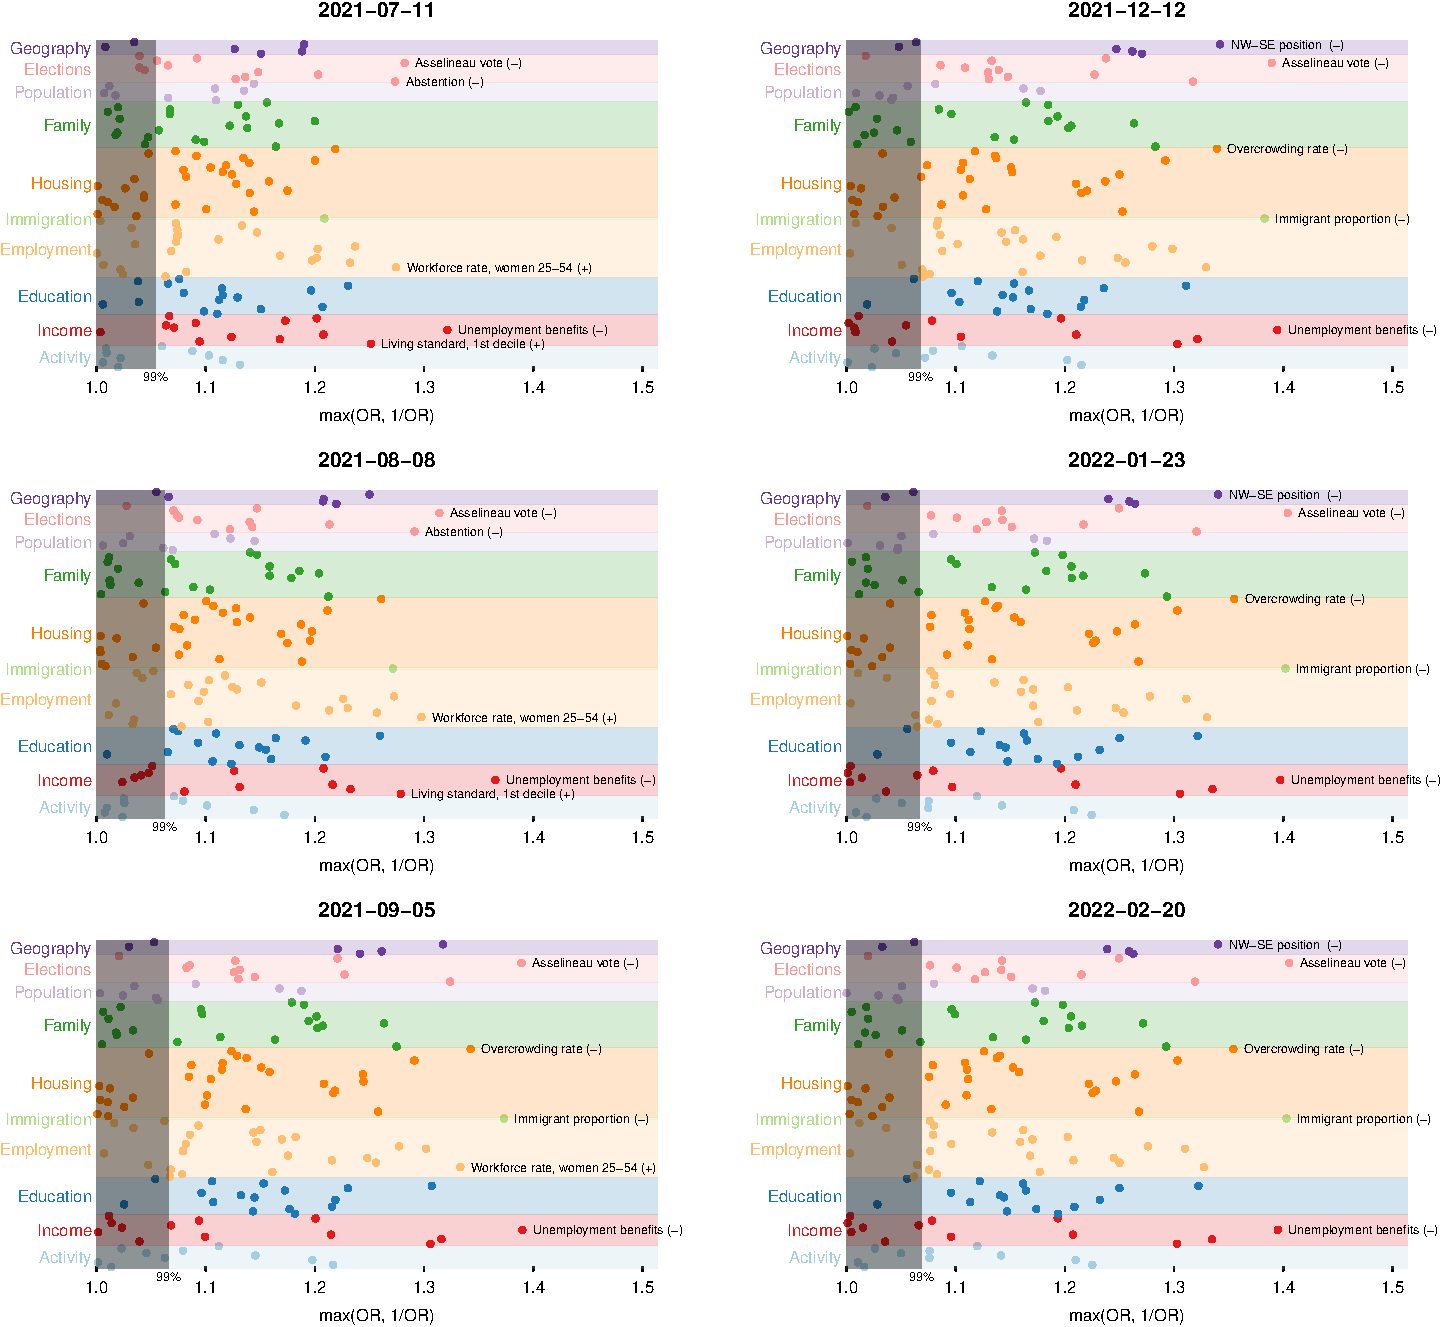
\includegraphics{figs_files/figure-latex/figManhattan-1.pdf}
\caption{\label{fig:figManhattan}Manhattan plots of the Odds ratios for each of the indicator of our dataset, by date. Left column: around the Sanitary Pass implementation; right column: around the Vaccine Pass implementation. The top odds ratios are labelled at each time point; the symbol next to the name indicates the direction of the effect. The gray rectangle corresponds to the 99\% percentile of odds ratios in the permuted data; points falling in the rectangle are considered as non-significant.}
\end{figure}

\begin{Shaded}
\begin{Highlighting}[]
\FunctionTok{plotManhattan}\NormalTok{(outLR, }\AttributeTok{ntop =} \DecValTok{5}\NormalTok{)}
\end{Highlighting}
\end{Shaded}

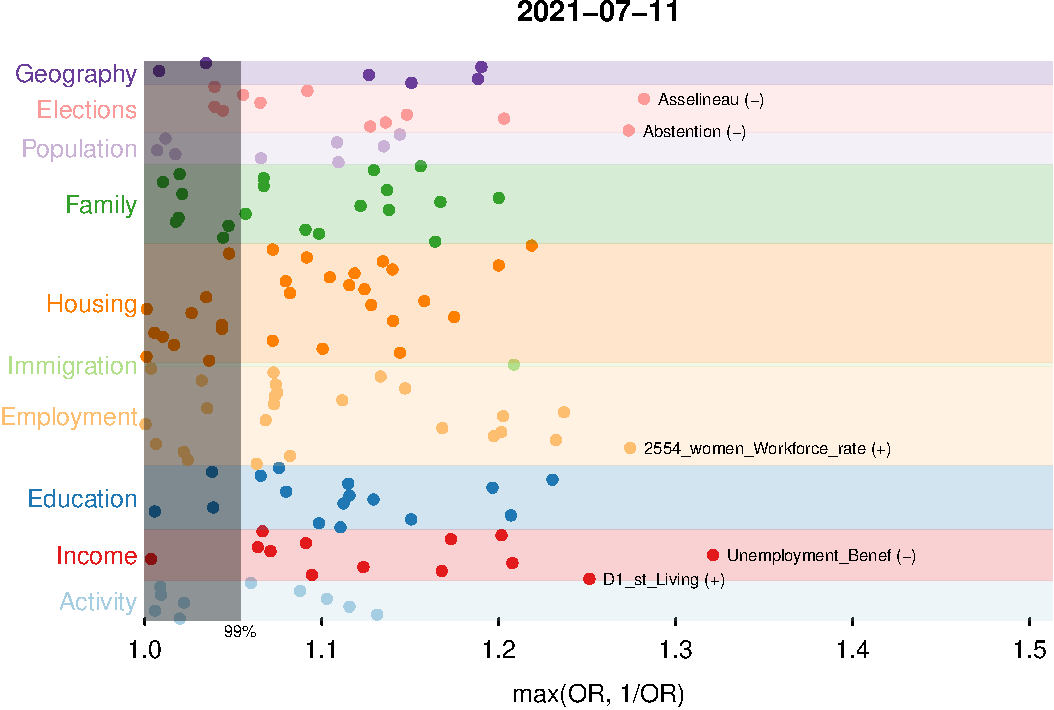
\includegraphics{figs_files/figure-latex/manhattanSingles-1.pdf} 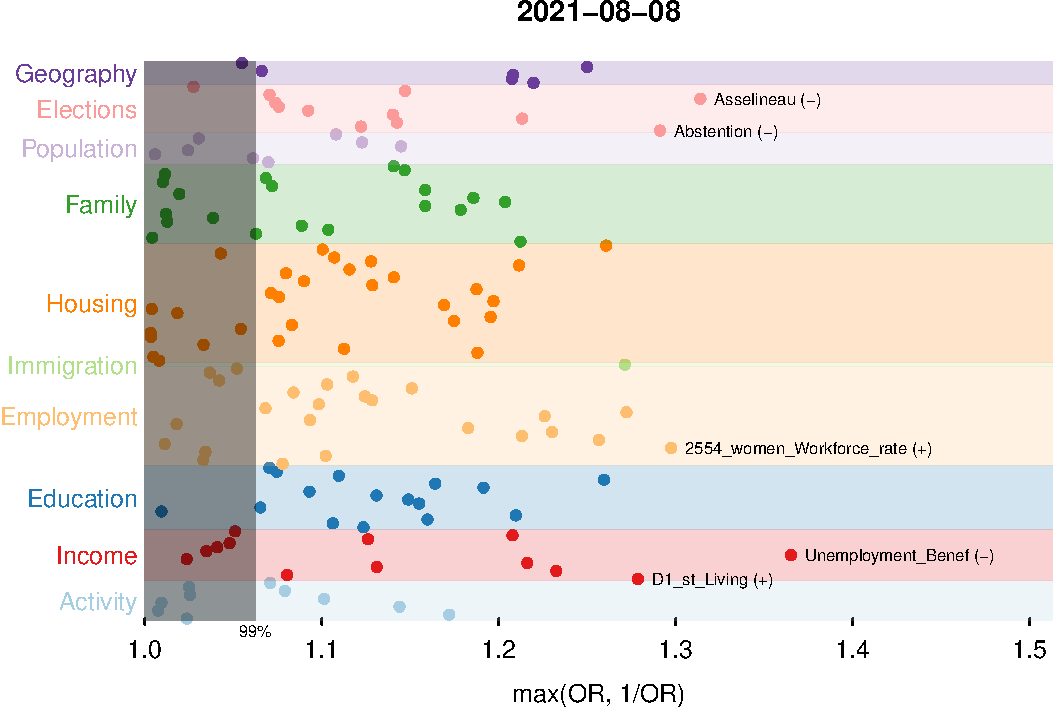
\includegraphics{figs_files/figure-latex/manhattanSingles-2.pdf} 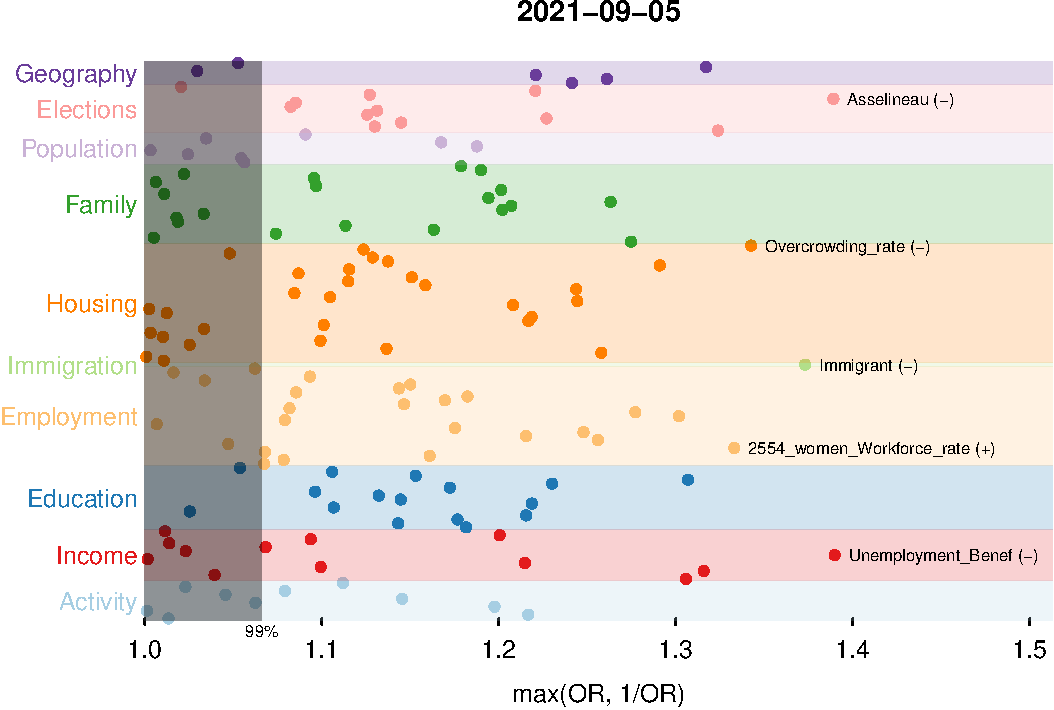
\includegraphics{figs_files/figure-latex/manhattanSingles-3.pdf} 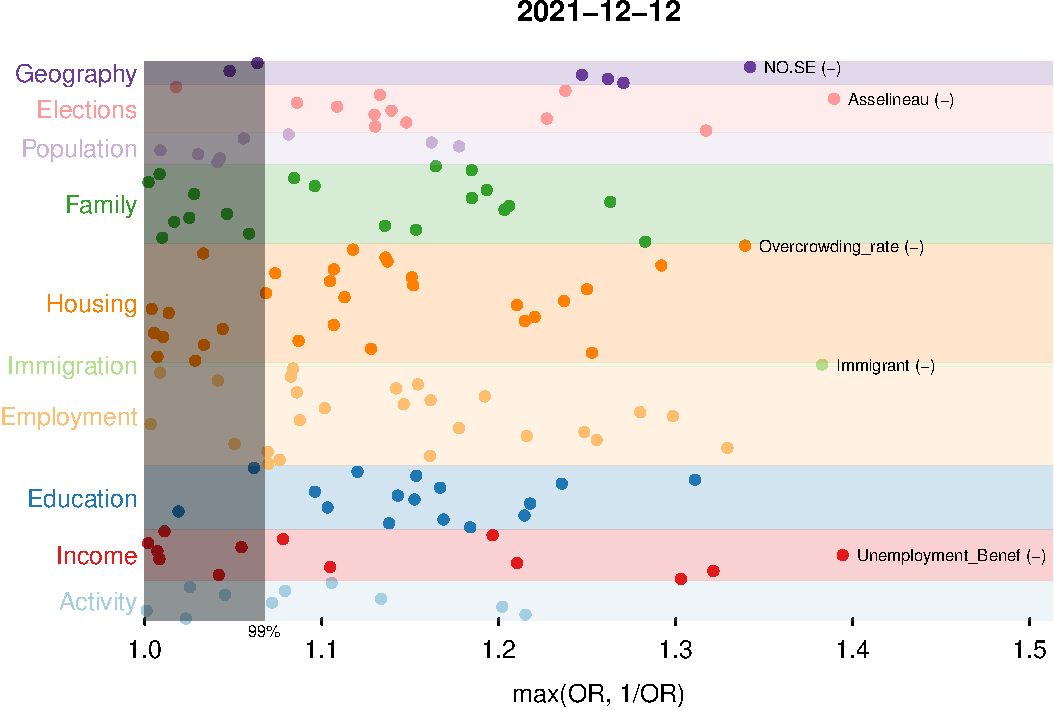
\includegraphics{figs_files/figure-latex/manhattanSingles-4.pdf} 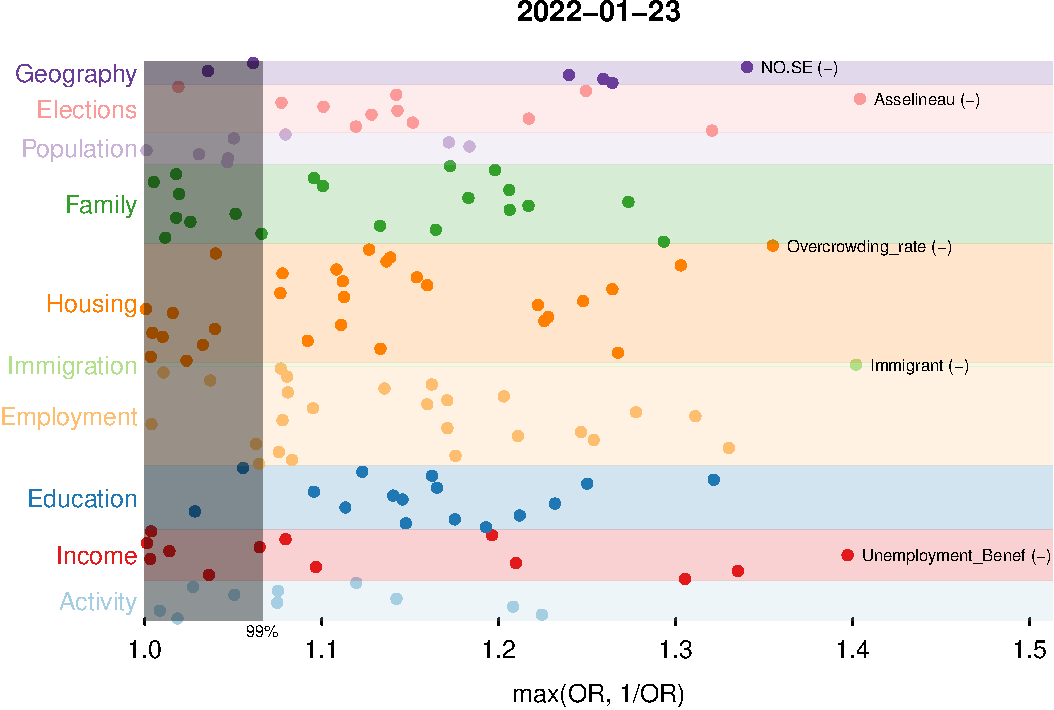
\includegraphics{figs_files/figure-latex/manhattanSingles-5.pdf} 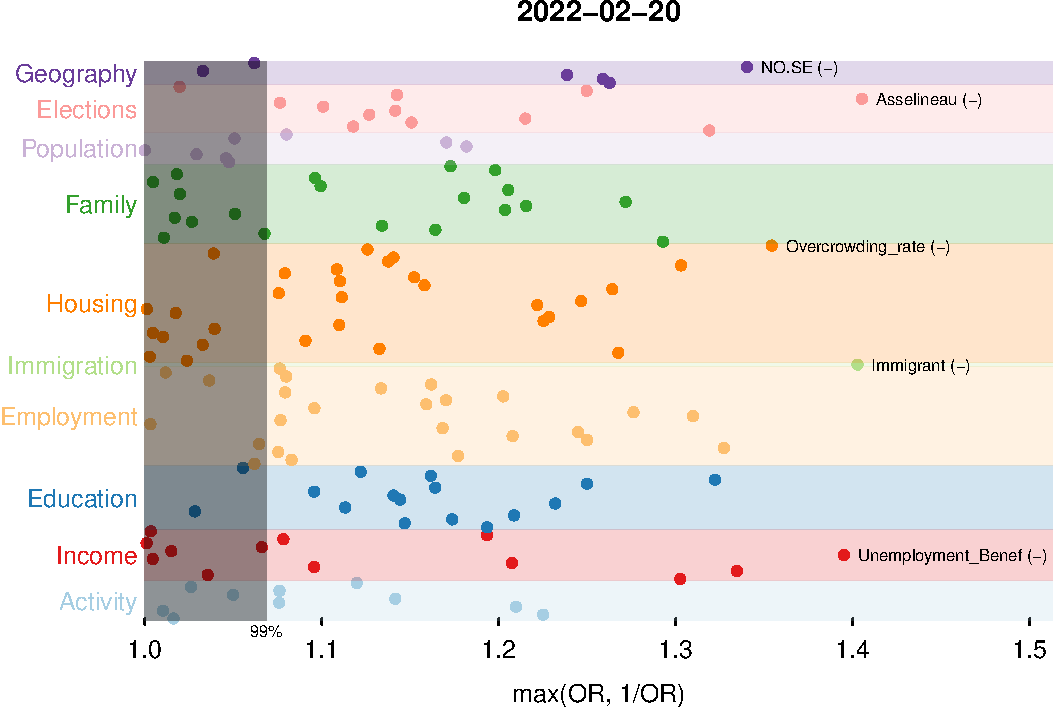
\includegraphics{figs_files/figure-latex/manhattanSingles-6.pdf}

\begin{figure}
\centering
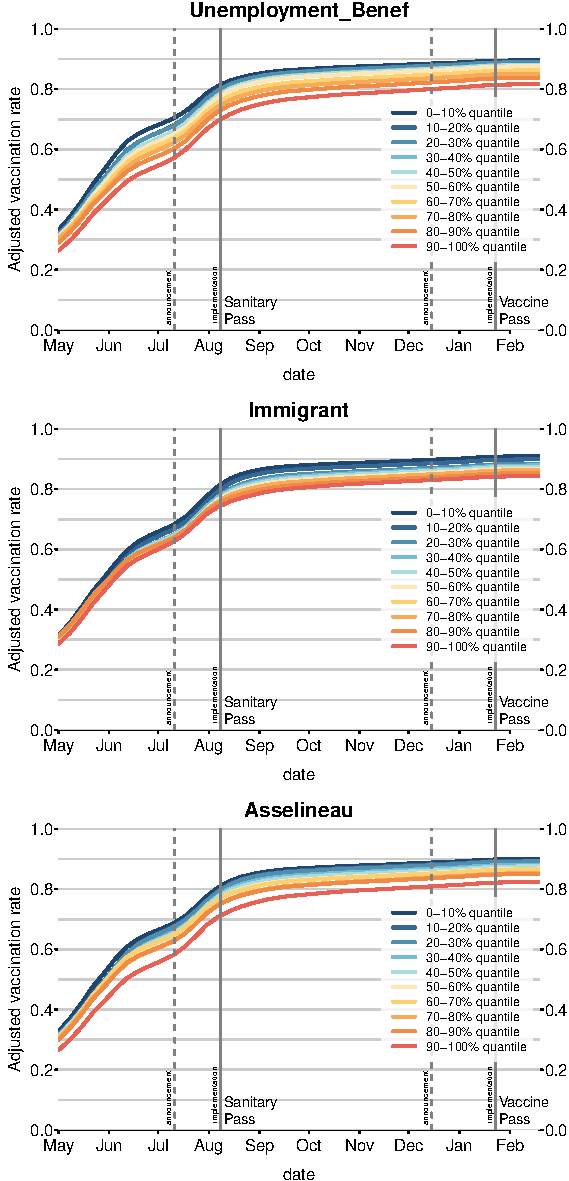
\includegraphics{figs_files/figure-latex/figOverTime-1.pdf}
\caption{\label{fig:figOverTime}Age-adjusted vaccination rates among adults, over time, by decile of each indicator (presented by a color gradient). The vertical lines indicate the dates of announcements and implementations of the sanitary and vaccine passes.}
\end{figure}

\begin{Shaded}
\begin{Highlighting}[]
\FunctionTok{plotPropTime}\NormalTok{(outA, }\AttributeTok{plotDates =} \ConstantTok{TRUE}\NormalTok{, }\AttributeTok{plotGraduations =} \ConstantTok{TRUE}\NormalTok{)}
\end{Highlighting}
\end{Shaded}

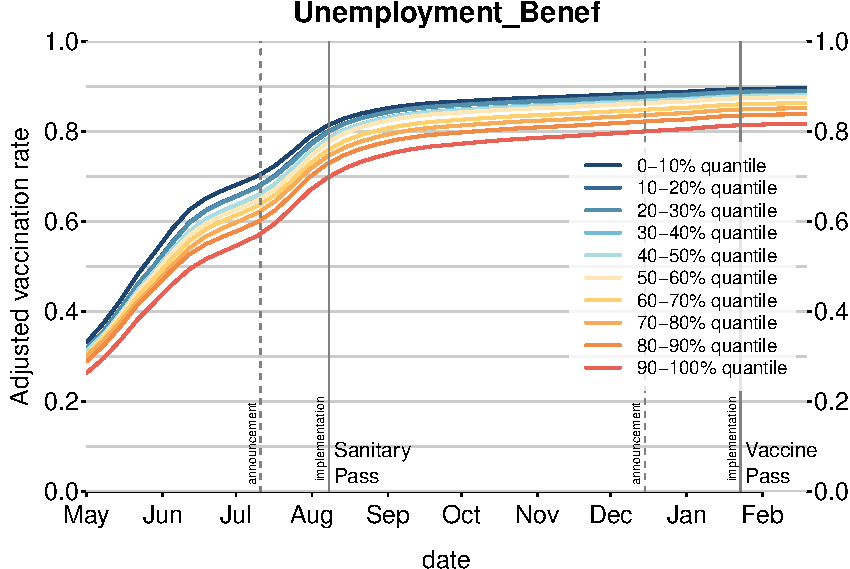
\includegraphics{figs_files/figure-latex/overTimeSingles-1.pdf} 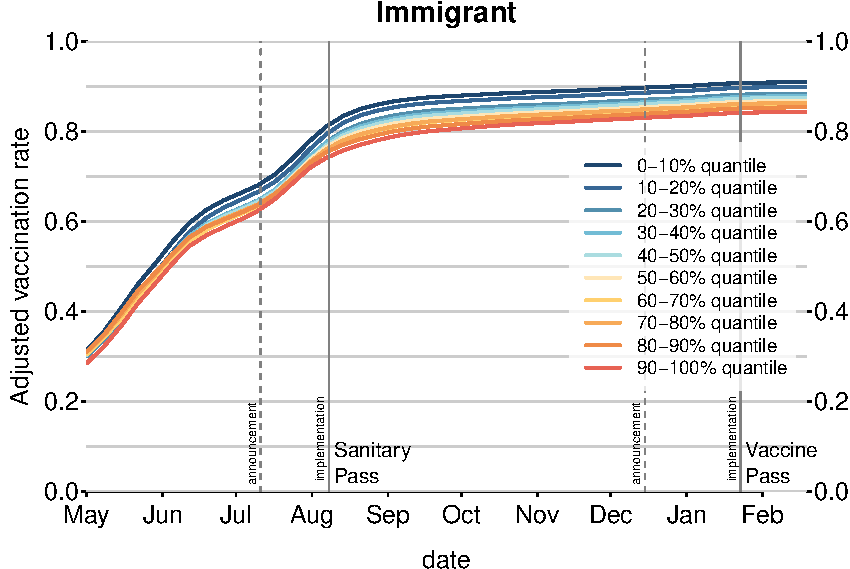
\includegraphics{figs_files/figure-latex/overTimeSingles-2.pdf} 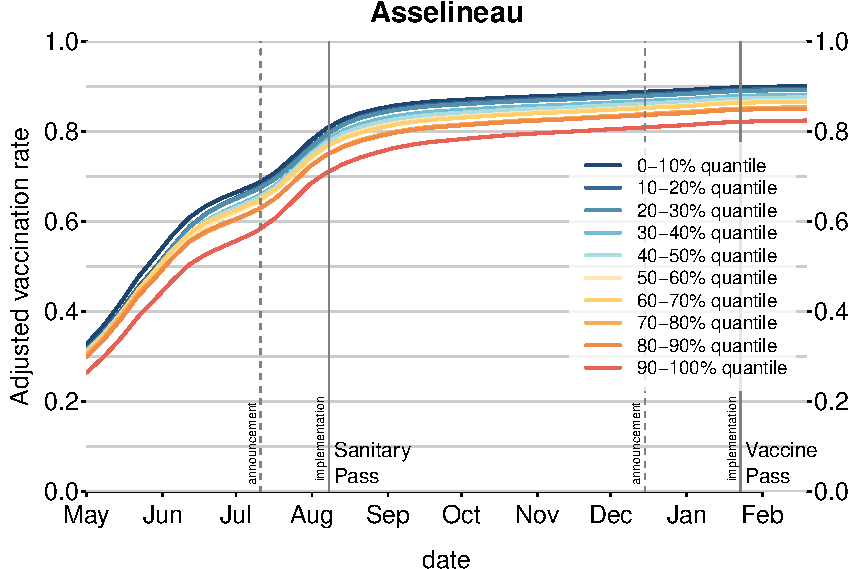
\includegraphics{figs_files/figure-latex/overTimeSingles-3.pdf}

\begin{figure}
\centering
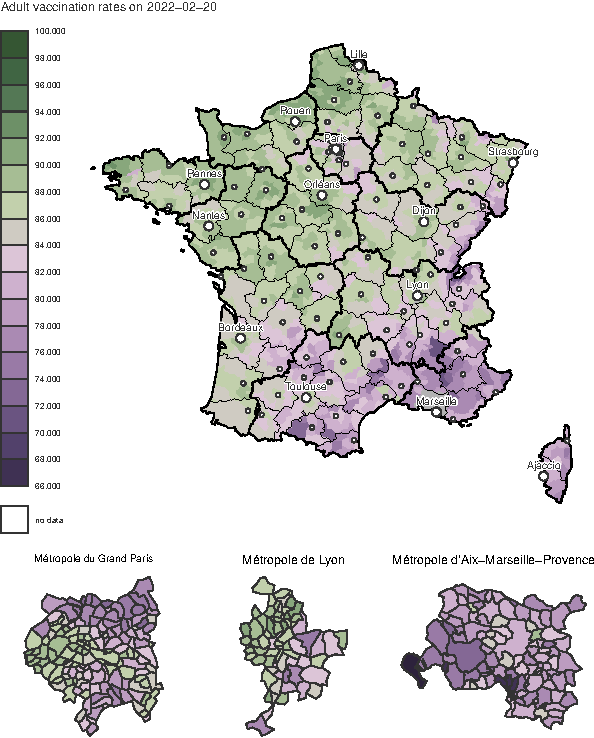
\includegraphics{figs_files/figure-latex/figMap-1.pdf}
\caption{\label{fig:figMap}Adult vaccination rates by district of mainland France}
\end{figure}

\end{document}
